% This file was created with tikzplotlib v0.10.1.
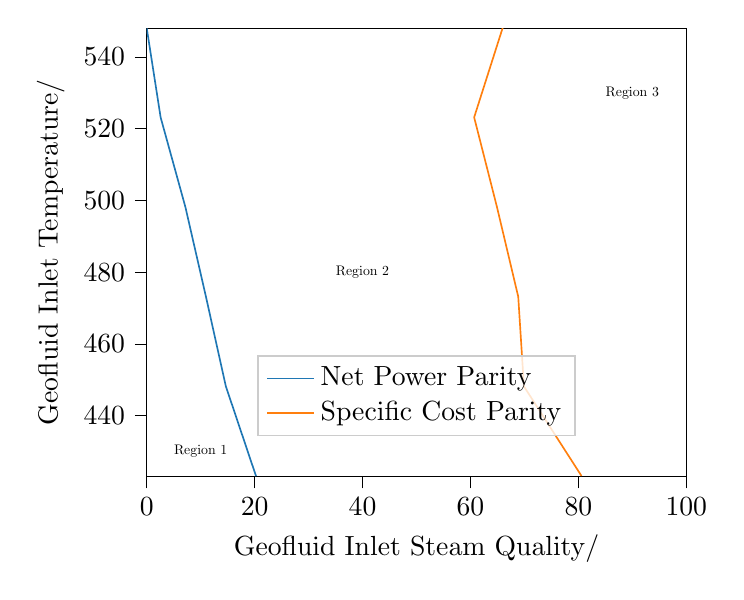
\begin{tikzpicture}

\definecolor{darkgray176}{RGB}{176,176,176}
\definecolor{darkorange25512714}{RGB}{255,127,14}
\definecolor{lightgray204}{RGB}{204,204,204}
\definecolor{steelblue31119180}{RGB}{31,119,180}

\begin{axis}[
legend cell align={left},
legend style={
  fill opacity=0.8,
  draw opacity=1,
  text opacity=1,
  at={(0.5,0.09)},
  anchor=south,
  draw=lightgray204
},
tick align=outside,
tick pos=left,
x grid style={darkgray176},
xlabel={Geofluid Inlet Steam Quality/\unit{\percent}},
xmin=0, xmax=100,
xtick style={color=black},
y grid style={darkgray176},
ylabel={Geofluid Inlet Temperature/\unit{\K}},
ymin=423, ymax=548,
ytick style={color=black}
]
\addplot [semithick, steelblue31119180]
table {%
20.2574810001872 423.15
14.6736248492937 448.15
10.9828903695487 473.15
7.17456971654515 498.15
2.5857550533881 523.15
0 548.15
};
\addlegendentry{Net Power Parity}
\addplot [semithick, darkorange25512714]
table {%
80.5840390695152 423.15
69.9083413304653 448.15
68.8529408109643 473.15
64.9111763437638 498.15
60.6841000655588 523.15
65.9803998207952 548.15
};
\addlegendentry{Specific Cost Parity}
\draw (axis cs:10,430) node[
  scale=0.5,
  text=black,
  rotate=0.0
]{Region 1};
\draw (axis cs:40,480) node[
  scale=0.5,
  text=black,
  rotate=0.0
]{Region 2};
\draw (axis cs:90,530) node[
  scale=0.5,
  text=black,
  rotate=0.0
]{Region 3};
\end{axis}

\end{tikzpicture}
